\documentclass[10pt,twocolumn,letterpaper]{article}

\usepackage{iccv}
\usepackage{times}
\usepackage{epsfig}
\usepackage{graphicx}
\usepackage{amsmath}
\usepackage{amssymb}
\usepackage{mathrsfs}
\usepackage{mathtools}
\usepackage{subfigure}
\usepackage{multirow}
\usepackage{epstopdf}

\DeclareMathOperator*{\argmin}{arg\,min}
% Include other packages here, before hyperref.

% If you comment hyperref and then uncomment it, you should delete
% egpaper.aux before re-running latex.  (Or just hit 'q' on the first latex
% run, let it finish, and you should be clear).
\usepackage[pagebackref=true,breaklinks=true,letterpaper=true,colorlinks,bookmarks=false]{hyperref}

\newcommand{\deva}[1]{\textcolor{blue}{[Deva: #1]}}
\newcommand{\new}[1]{\textcolor{red}{#1}}
\newcommand{\songfan}[1]{\textcolor{blue}{[Songfan: #1]}}

\def\iccvPaperID{1416} % *** Enter the ICCV Paper ID here
\def\httilde{\mbox{\tt\raisebox{-.5ex}{\symbol{126}}}}

% Pages are numbered in submission mode, and unnumbered in camera-ready
\ificcvfinal\pagestyle{empty}\fi
\begin{document}

%%%%%%%%% TITLE
\title{Multi-scale recognition with DAG-CNNs}

\author{Songfan Yang\\
College of Electronics and Information Engineering,\\
Sichuan University, China\\
{\tt\small syang@scu.edu.cn}
% For a paper whose authors are all at the same institution,
% omit the following lines up until the closing ``}''.
% Additional authors and addresses can be added with ``\and'',
% just like the second author.
% To save space, use either the email address or home page, not both
\and
Deva Ramanan\\
Deptment of Computer Science,\\
University of California, Irvine, USA\\
{\tt\small dramanan@ics.uci.edu}
}

\maketitle
%\thispagestyle{empty}


%%%%%%%%% ABSTRACT
\begin{abstract}
We explore multi-scale convolutional neural nets (CNNs) for image classification. Contemporary approaches extract features from a single output layer. By extracting features from multiple layers, one can simultaneously reason about high, mid, and low-level features during classification. The resulting multi-scale architecture can itself be seen as a feed-forward model that is structured as a directed acyclic graph (DAG-CNNs). %We show that DAG-CNNs are just as fast as chain-structured CNNs in terms of training and testing. In fact, training is easier because multi-scale connections tend to minimize the vanishing gradient problem. 
We use DAG-CNNs to learn a set of multi-scale features that can be effectively shared between coarse and fine-grained classification tasks. While fine-tuning such models helps performance, we show that even ``off-the-self'' multi-scale features perform quite well. We present extensive analysis and demonstrate state-of-the-art classification performance on three standard scene benchmarks (SUN397, MIT67, and Scene15). %and show  state-of-the-art classification performance on all benchmarks., %\ie 55.5\% on SUN397, 76.1\% on MIT67, and 92.4\% on Scene15.
%\ie 56.2\% on SUN397, 77.5\% on MIT67, and 92.9\% on Scene15. 
In terms of the heavily benchmarked MIT67 and Scene15 datasets, our results reduce the lowest previously-reported error by {\bf 23.9\%} and {\bf 9.5\%}, respectively.
\end{abstract}

%%%%%%%%% BODY TEXT
\section{Introduction}


\begin{figure}[t!]
\centering
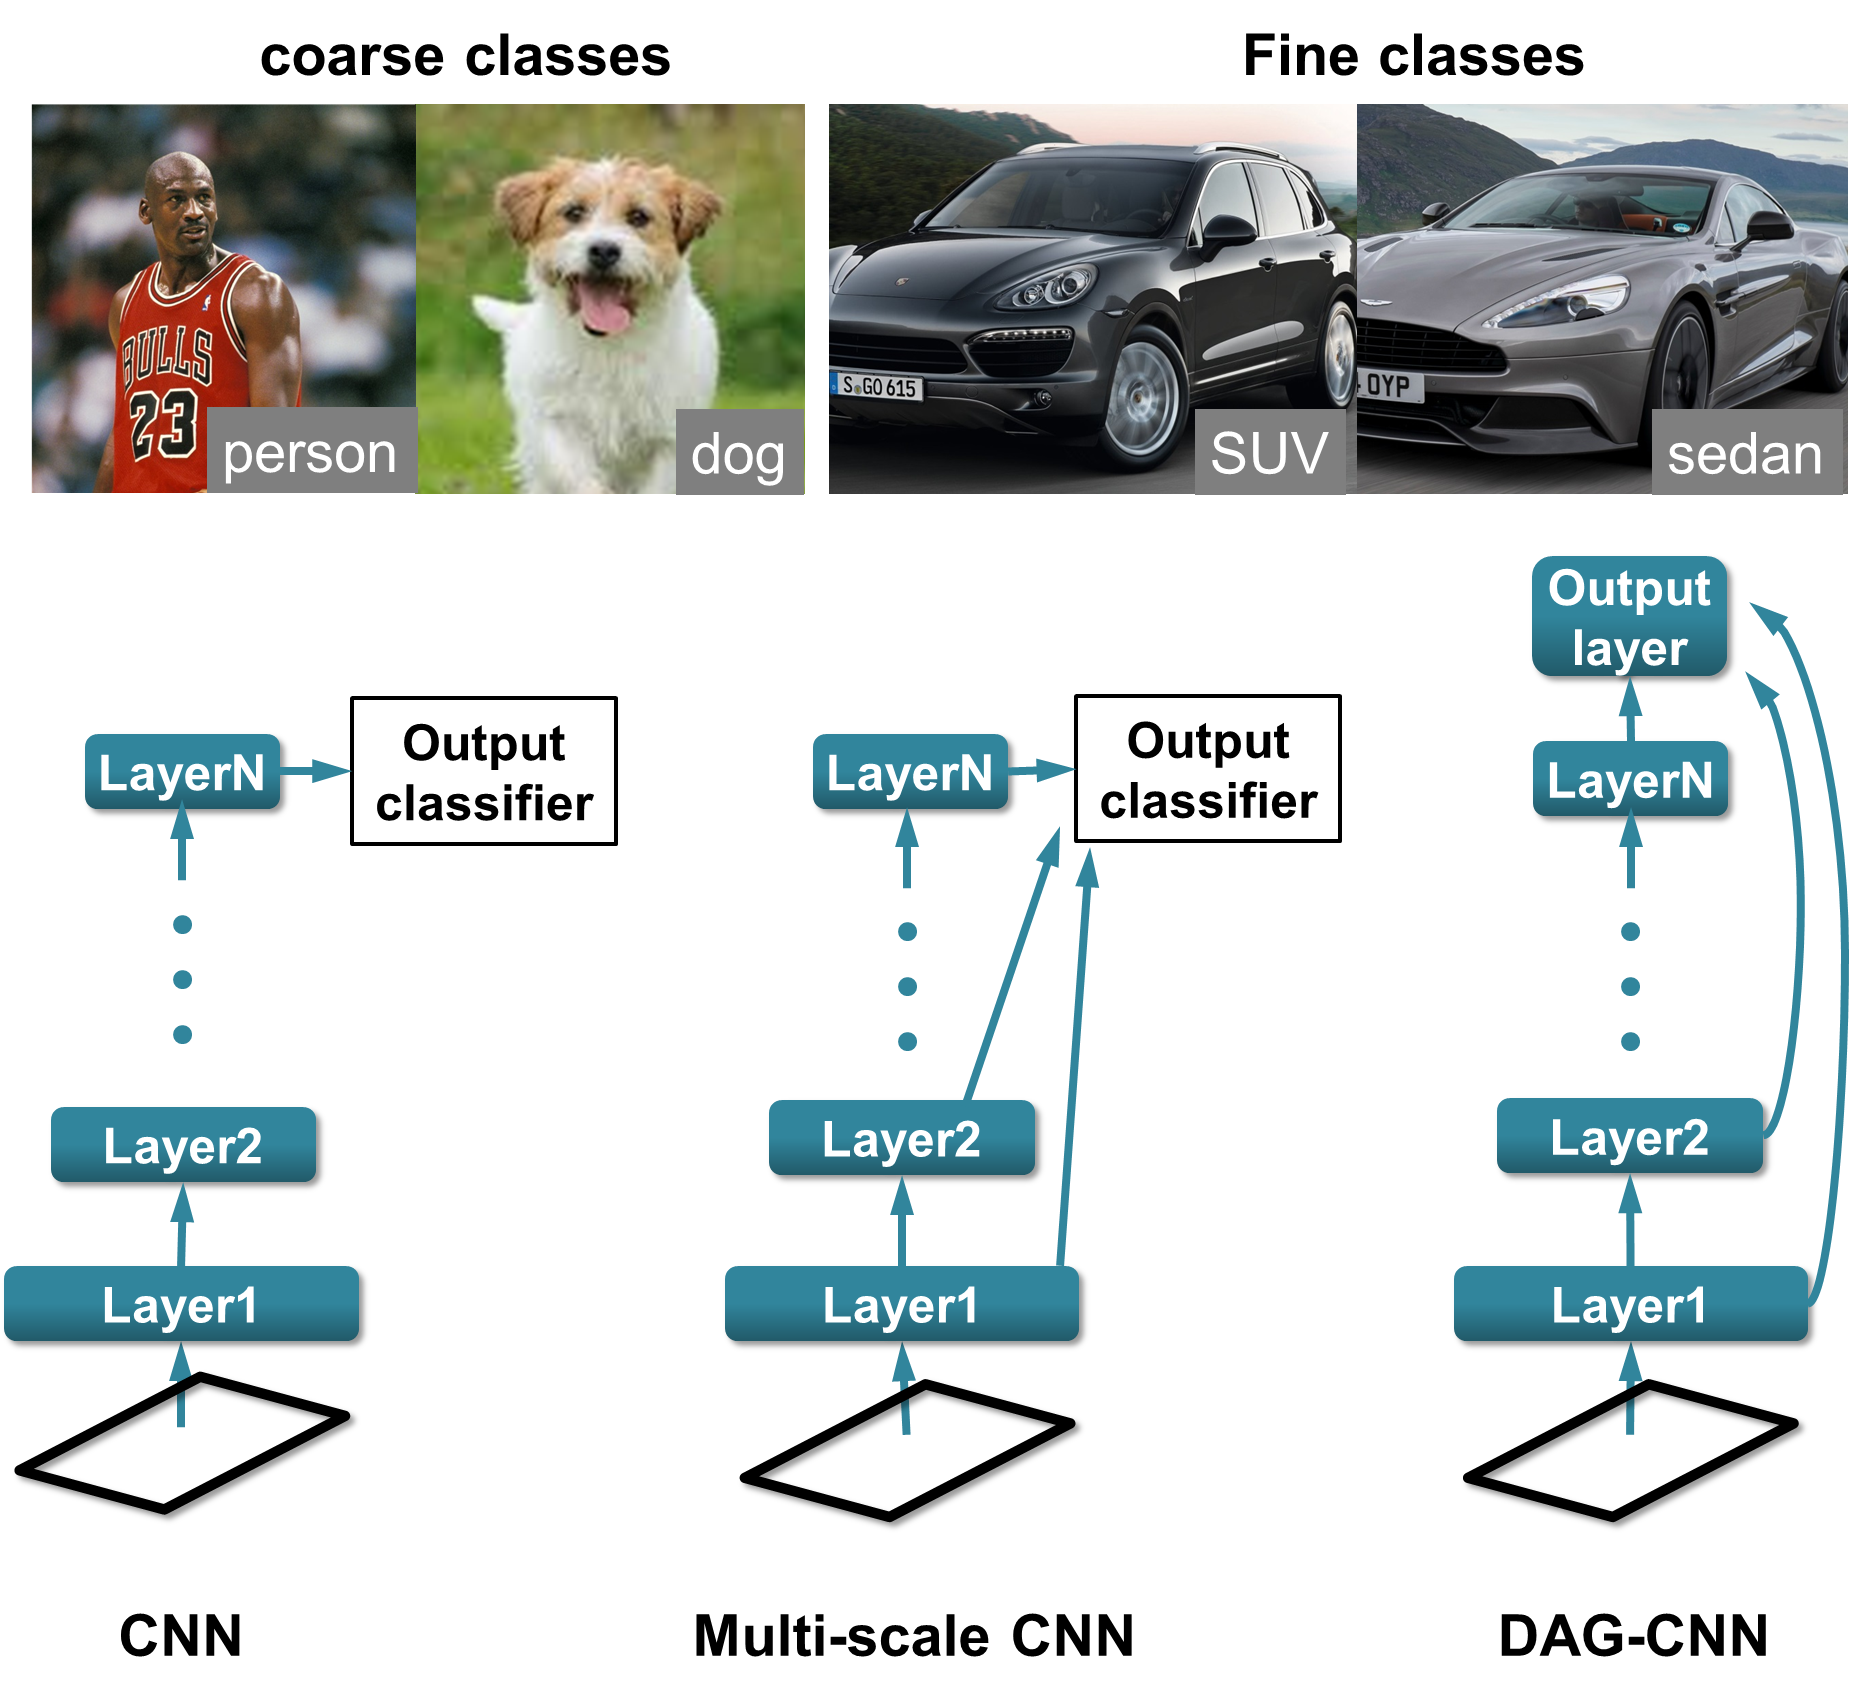
\includegraphics[width=\columnwidth]{fig/splash}
\caption{Recognition typically require features at multiple scales. Distinguishing a person versus dog requires highly invariant features robust to the deformation of each category. On the other hand, fine-grained recognition likely requires detailed shape cues to distinguish models of cars ({\bf top}). We use these observations to revisit deep convolutional neural net (CNN) architectures. Typical approaches train a classifier using features from a single output layer ({\bf left}). We extract multi-scale features from multiple layers to simultaneously distinguish coarse and fine classes. Such features come ``for free'' since they are already computed during the feed-forward pass ({\bf middle}). Interestingly, the entire multi-scale predictor is still a feed-forward architecture that is no longer chain-structured, but a directed-acyclic graph (DAG) ({\bf right}). We show that DAG-CNNs can be discriminatively trained in an end-to-end fashion, yielding state-of-the-art recognition results across various recognition benchmarks. }% DAG-CNNs address some well-known challenges with CNNs such as ``vanishing gradients''~\cite{bengio1994learning}. Lower layers in a DAG-CNN still receive a strong gradient signal during learning because they are directly tied to the output layer, making them easier to train.
\label{fig:splash}
\end{figure}

Deep convolutional neural nets (CNNs), pioneered by Lecun and collaborators~\cite{lecun1998gradient}, now produce state-of-the-art performance on many visual recognition tasks~\cite{AlexNet, veryDeep, GoogLeNet}. An attractive property is that it appear to serve as universal feature extractors, either as ``off-the-shelf'' features or through a small amount of ``fine tuning''. CNNs trained on particular tasks such as large-scale image classification~\cite{ImageNet} {\em transfer} extraordinarily well to other tasks such as object detection~\cite{rcnn}, scene recognition~\cite{zhoulearning}, image retrieval~\cite{Gong14}, etc \cite{cnn_baseline}.

{\bf Hierarchical chain models:}  CNNs are 
hierarchical feed-forward architectures that compute progressively invariant representations of the input image. However, the appropriate level of invariance might be task-dependent. Distinguishing people and dogs requires a representation that is robust to large spatial deformations, since people and dogs can articulate. However, fine-grained categorization of car models (or bird species) requires fine-scale features that capture subtle shape cues. We argue that a universal architecture capable of both tasks must employ some form of multi-scale features for output prediction.

\begin{figure*}
\centering
	\subfigure[mid-level feature is preferred]{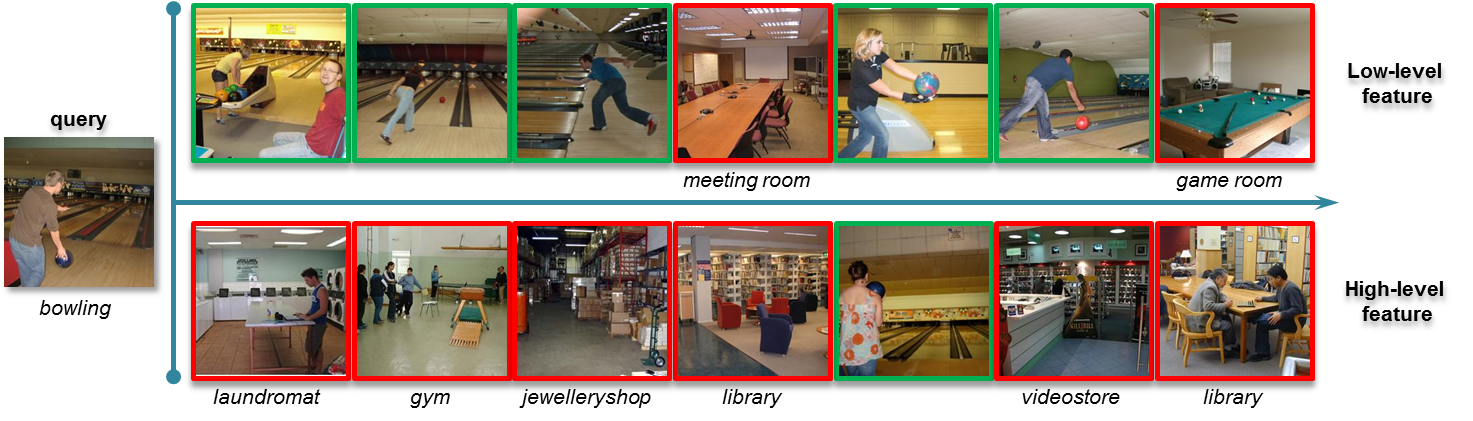
\includegraphics[height=.245\textwidth]{fig/moti_low_better}\label{fig:moti_low}}
	\subfigure[high-level feature is preferred]{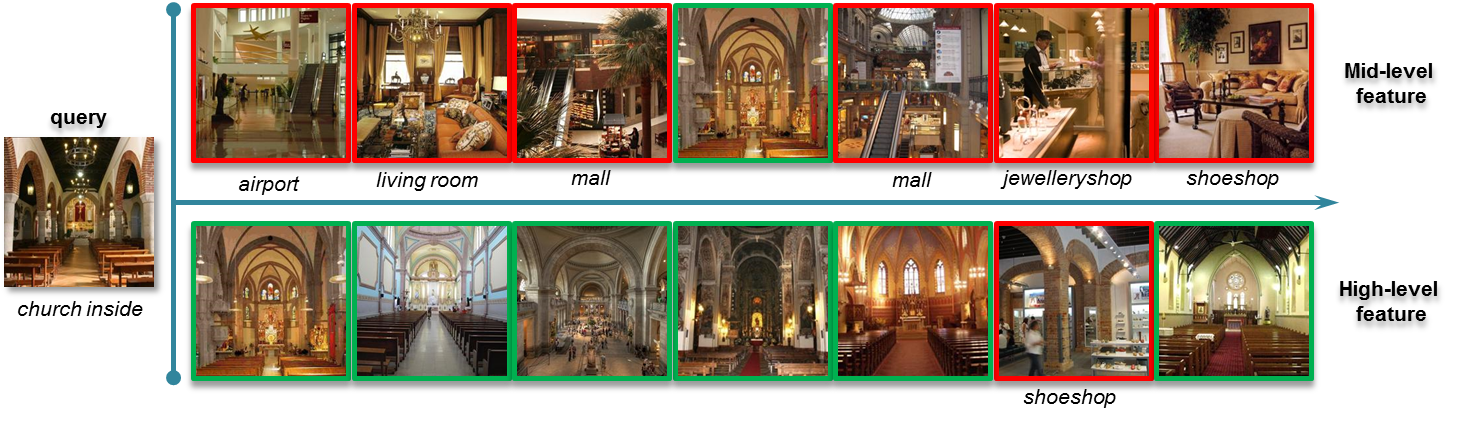
\includegraphics[height=.245\textwidth,clip=true,trim=23mm 0mm 0mm 0mm]{fig/moti_high_better}\label{fig:moti_high}}
%	\subfigure[mid-level feature is preferred]{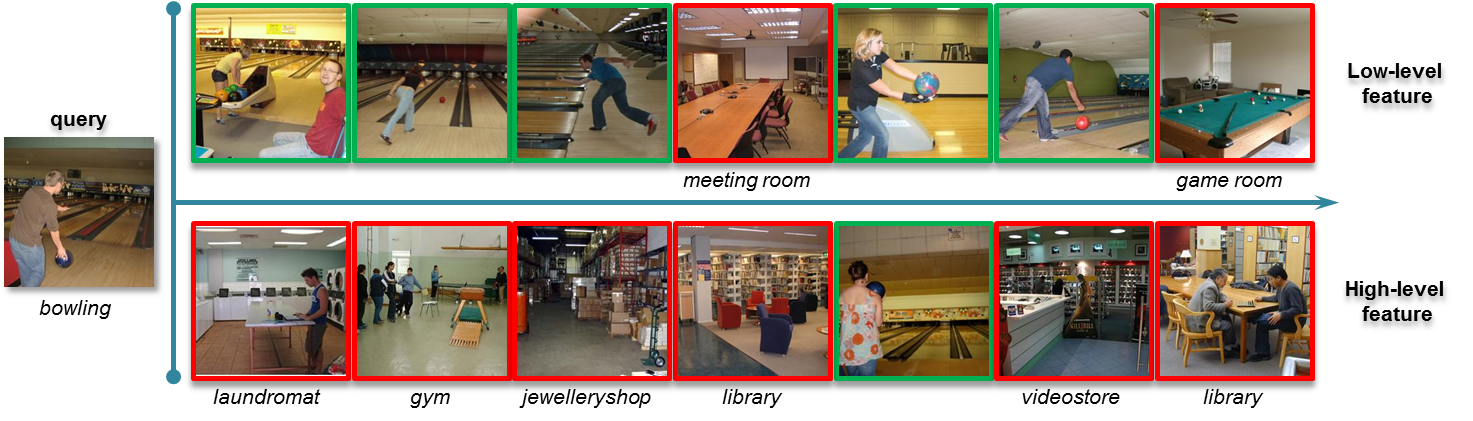
\includegraphics[width=.49\textwidth]{fig/moti_low_better}\label{fig:moti_low}}
%	\subfigure[high-level feature is preferred]{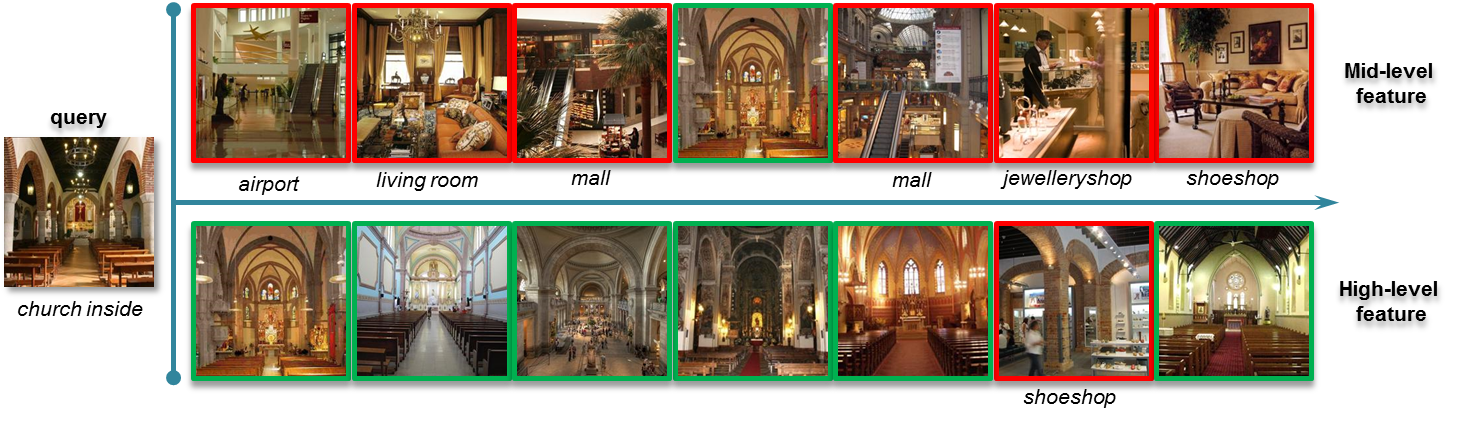
\includegraphics[width=.49\textwidth]{fig/moti_high_better}\label{fig:moti_high}}
\caption{Retrieval results using L2 distance for both mid- and high-level features on MIT67~\cite{MIT67}, computed from layer 11 and 20 of the Caffe model. \textit{Green} (\textit{Red}) box means correct (wrong) results, in terms of the scene category label. The correct label for wrong retrievals are provided. The retrieval results are displayed such that the left-most image has the closest distance to the query, and vice versa. Certain query images (or categories) produce better matches with high-level features, while others produce better results with mid-level features. This motivates our multi-scale approach.}
\label{fig:moti}
\end{figure*}


{\bf Multi-scale representations:}  Multi-scale representations are a classic concept in computer vision, dating back to image pyramids~\cite{burt1983laplacian}, scale-space theory ~\cite{lindeberg1993scale}, and multi-resolution models~\cite{mallat1999wavelet}. Though somewhat fundamental notions, they have not been tightly integrated with contemporary feed-forward approaches for recognition. We introduce multi-scale CNN architectures that use features at multiple scales for output prediction (Fig.~\ref{fig:splash}). From one perspective, our architectures are quite simple. Typical approaches train a output predictor (e.g., a linear SVM) using features extracted from a single output layer. Instead, one can train an output predictor using features extracted from {\em multiple} layers. Note that these features come ``for free''; they are already computed in a standard feed-forward pass.

{\bf Spatial pooling:} One difficulty with multi-scale approaches is feature dimensionality - the total number of features across all layers can easily reach hundreds of thousands. This makes training even linear models difficult and prone to over-fitting. Instead, we use marginal activations computed from sum (or max) pooling across spatial locations in a given activation layer. From this perspective, our models are similar to those that compute multi-scale features with spatial pooling, including multi-scale templates~\cite{felzenszwalb2008discriminatively}, orderless models~\cite{Gong14}, spatial pyramids~\cite{spatial_pyramid}, and bag-of-words~\cite{sivic2003video}. Our approach is most related to~\cite{Gong14}, who also use spatially pooled CNN features for scene classification. They do so by pooling together multiple CNN descriptors (re)computed on various-sized patches within an image. Instead, we perform a single CNN encoding of the entire image, extracting multi-scale features ``for free''.

{\bf End-to-end training:} Our multi-scale model differs from such past work in another notable aspect. Our entire model is still a feed-forward CNN that is no longer chain-structured, but a directed-acyclic graph (DAG). DAG-structured CNNs can still be discriminatively trained in an end-to-end fashion, allowing us to directly learn multi-scale representations. %Multi-scale learning addresses one well-known difficulty of CNNs - the ``vanishing gradient'' problem~\cite{bengio1994learning}. During gradient-based learning, the gradient signal becomes progressively diluted as one back-propagates it through multiple layers, such that the bottom-most layer receives essentially no updates. Our multi-scale DAG structure connects all activation layers directly to the output, ensuring they all receive a strong gradient signal during learning.  
DAG structures are relatively straightforward to implement given the flexibility of many deep learning toolboxes~\cite{vedaldimatconvnet,Caffe}. Our primary contribution is the demonstration that structures can capture multi-scale features, which in turn allow for transfer learning between coarse and fine-grained classification tasks.

%yeilding state-of-the-art recognition results across various recognition benchmarks. 

% Trained with large number of instances, (such as ImageNet~\cite{ImageNet}), CNN is also an excel candidate for off-the-shelf feature extractions, results in outstanding performance in various recognition tasks~\cite{cnn_baseline}. In the meantime, a considerable amount of effort is spent on how to further improve the performance of CNN. On one hand, many are focus on techniques to efficiently and effective train a CNN. A good initialization need to be carefully selected~\cite{diff_cnn} in the beginning. Data augmentation~\cite{AlexNet} is recommended to improve the model performance as well. Drop-out~\cite{dropout} and momentum~\cite{momentum} are also necessary to prevent over-fitting and obtain superior models. On the other hand, different model components and architectures are proposed. Rectified linear units (ReLU)~\cite{AlexNet} add non-linearity and enrich the model complexity. Different pooling method, such as Distance Transform Pooling~\cite{dist_trans}, is adopted in~\cite{dpm_is_cnn}, allowing local deformations, as in the widely-used deformable part-based model (DPM)~\cite{dpm}. \cite{veryDeep} adopts a small $3\times 3$ receptive field to deepen the model, while maintaining less parameters. A network in network~\cite{nin} is proposed to enhance model discriminability for local patches within the receptive field. The award winning GoogLeNet~\cite{GoogLeNet} uses an \textit{Inception} model that is based on the Hebbian principle~\cite{Hebb}, \ie, neurons that fire together, wire together, the theoretical proof of which is provided by~\cite{dnn_proof} under constraints. 

%One question to ponder: is there any model-independent potential that is yet to be discovered. Although allowing local deformation, CNN encodes the the spatial information of multi-scale features. Conversely, by ignoring the spatial location of features, bag-of-feature like techniques~\cite{spatial_pyramid} achieves transformation invariance to some extend. As pointed out in~\cite{Gong14}, combining both type of features results in a better representation for recognition tasks with large variations, such as Scene classification~\cite{SUN397,MIT67}. Traditionally, when CNN is used for feature extraction, the activation of the first fully-connected (FC) layer is usually considered as the feature~\cite{overfeat, Gong14}. Using an off-the-shelf deep CNN model,~\cite{Gong14} explicitly extracts image patches from three scales and computes the feed-forward CNN activations for each patch for feature extraction. This algorithm is cumbersome due to the computation of multiple patches for one image. Besides, it can only encode the multi-scale features to a certain extend limited by the burden of the post processing, \ie, K-means and Principle Component Analysis (PCA). As a matter of fact, CNN feature is meant to encode multi-scale feature at each convolutional (Conv.) layer. Therefore, there is no need to extract multi-scale patches and only one feed-forward computation is sufficient to capture the activations of multi-scale features for one input image. 


%In this paper, we first conducted an empirical analysis on the feature discriminativeness of every unit of CNN model. By average-pooling at each layer, the output ignores global spatial information and results in a bag-of-feature representation. The bag-of-feature from ReLU is then found to carry the most performance gain at each layer. We have also observed a synergy of multi-scale activations results in a better discriminative representation. These observations tie closely to the vanishing gradient~\cite{diff_cnn} issue in the deep CNN literature. During the training of a CNN, the top layer can be easily saturated. The gradients in the back-propagation algorithm will not effective reach the lower levels, resulting in a model that focuses more high-level features. Thus, we proposed a model augmentation schema, BoMSA, that chains the ReLU at each layer to the ultimate loss function. This augmentation approach is not confined by model variations and can be applied to existing pre-trained models or re-training the model from the ground up. By explicitly linking the lower layers to the decision layer, we gear the training towards the bag-of-activations from all layers. Thus, the augmented model is designed to be robust to spatial translations while maintaining its discriminative power in the multi-scale fashion.

{\bf DAG Neural Networks:} DAG-structured neural nets were explored earlier in the context of recurrent neural nets \cite{baldi2003principled,graves2009offline}. Recurrent neural nets use feedback to capture dynamic states, and so typically cannot be processed with feed-forward computations. %Previous work has also shown that long-range connections between neural layers can eliminate the vanishing gradient problem, but this is done in the context of memory-based networks~\cite{hochreiter1997long}. We make use of DAG structures to efficiently encode multi-scale features in a simpler feed-forward network. 
%{\bf Skip connections:} 
More recently, networks have explored the use of ``skip'' connections between layers \cite{raiko-aistats-12,GoogLeNet,sermanet2013pedestrian}, similar to our multi-scale connections. \cite{raiko-aistats-12} show that such connections are useful for a single binary classification task, but we motivate multi-scale connections through multi-task learning: different visual classification tasks require features at different image scales. %Indeed, we show that off-the-shelf multi-scale features transfer extraordinary well between classification tasks. 
Finally, the recent state-of-the-art model of \cite{GoogLeNet} make use of skip connections for training, but does not use them at test-time. This means that their final feedforward predictor is not a DAG. Our results suggest that adding multi-scale connections at test time might further improve their performance.
%multiscale features at test-time might further improve their performance.

{\bf Overview:} We motivate our multi-scale DAG-CNN model in Sec.~\ref{sec:motivation}, describe the full architecture in Sec.~\ref{sec:approach}, and conclude with numerous benchmark results in Sec.~\ref{sec:exp}. We evaluate multi-scale DAG-structured variants of existing CNN architectures (\eg, Caffe~\cite{Caffe}, Deep19~\cite{veryDeep}) on a variety of scene recognition benchmarks including SUN397~\cite{SUN397}, MIT67~\cite{MIT67}, Scene15~\cite{Scene15}. We observe a consistent improvement regardless of the underlying CNN architecture, producing state-of-the-art results on all 3 datasets.

%A consistent performance improvement is observed of our multi-scale representation over the best discriminative single-scale feature. 
%The rest of the paper is organized as follows: we motivate and describe our model augmentation approach in Sec.~
%\ref{sec:approach}. An in-depth analysis is provided in Sec.~\ref{sec:ana}. Systematic experimental results are included in Sec.~\ref{sec:exp}. 


%-------------------------------------------------------------------------
%-------------------------------------------------------------------------
\section{Motivation\label{sec:motivation}}

In this section, we motivate our multi-scale architecture with a series of empirical analysis. We carry out an analysis on existing CNN architectures, namely Caffe and Deep19. Caffe~\cite{Caffe} is a broadly used CNN toolbox. It includes a pre-trained model ``AlexNet''~\cite{AlexNet} model, learned with millions of images from the ImageNet dataset~\cite{ImageNet}. \new{We denote the output of each convolution, rectification, normalization, pooling, and fully-connected inner product operation as a unique layer. Under this definition, the Caffe AlexNet model has 20 layers, while the state-of-the-art Deep19 model ~\cite{veryDeep} has a total of 43 layers.}
% for a total of 20 layers.
%This model has 20 layers in total, including 6 conv. layers and 2 fully-connected (FC) layers. Deep19~\cite{veryDeep} uses very small $3\times 3$ receptive fields, but an increased number of layers -- 43 layers including 16 conv. and 3 FC layers.} This model produced state-of-the-art performance in ILSVRC-2014 classification challenge~\cite{ILSVRC14}. 
To develop our motivation, we analyze the behavior of the ``off-the-shelf'' Caffe model on the heavily benchmarked MIT Indoor Scene (MIT67) dataset~\cite{MIT67}, using 10-fold cross-validation.

\subsection{Single-scale models} 
%We first verify our hypothesis that different recognition tasks require different amounts of invariance through two experiments.

{\bf Image retrieval:} Recent work has explored sparse reconstruction techniques for visualizing and analyzing features~\cite{vondrick2013hoggles}. Inspired by such techniques, we use image retrieval to begin our exploration. We attempt to ``reconstruct'' a query image by finding $M=7$ closest images in terms of L2-distance, when computed with mean-pooled layer-specific activations. Results are shown for two query images and two Caffe layers in Fig.~\ref{fig:moti}. The {\tt florist} query image tends to produces better matches when using mid-level features that appear to capture \textit{objects} and \textit{parts}. On the other hand, the {\tt church-inside} query image tends to produce better matches when using high-level features that appear to capture more global \textit{scene} statistics.


%By working with poo providing some degree of robustness to spatial transformation of objects (bowling ball and people body parts). On the other hand, the example in Fig.~\ref{fig:moti_high} shows high-level feature captures the spatial geometry information. This is important for classes such as scenes with strong \textit{structure} cues, \eg, church, cloister, corridor, etc. Thus, we wish to develop a method that captures the multi-scale invariance.



%\subsection{Scale-specific classification}
%We carry out an analysis on existing CNN architectures, namely Caffe and Deep19. Caffe~\cite{Caffe} is a broadly used CNN toolbox. It includes a pre-trained model ``AlexNet''~\cite{AlexNet} model, learned with millions of images from the ImageNet dataset~\cite{ImageNet}. This model has 6 conv. layers and 2 fully-connected (FC) layers. Deep19~\cite{veryDeep} uses very small $3\times 3$ receptive fields, but an increased number of layers -- 19 layers (16 conv. and 3 FC layers). This model produced state-of-the-art performance in ILSVRC-2014 classification challenge~\cite{ILSVRC14}. We evaluate both models on the heavily benchmarked MIT Indoor Scene (MIT67) dataset~\cite{MIT67}.

\begin{figure}[t!]
\centering
	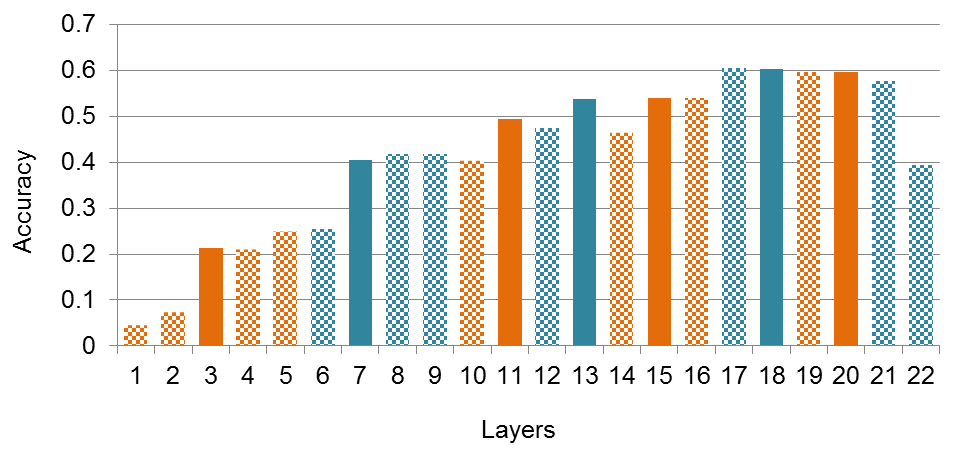
\includegraphics[width=.9\columnwidth]{fig/fig_layer_caffe}

\caption{The classification accuracy on MIT67~\cite{MIT67} using activations from each layer. We use an orange color fill representing the output of a ReLU layer, where there are 7 in total for the Caffe model. We tend to see a performance jump at each successive ReLU layer, particularly earlier on in the model.}
\label{fig:layer_MIT67}
\end{figure}

{\bf Single-scale classification:} Following past work \cite{cnn_baseline}, we train a linear SVM classifier using features extracted from a particular layer. We specifically train $K=67$ 1-vs-all linear classifiers.
We plot the performance of single-layer classifiers in Fig.~\ref{fig:layer_MIT67}. The detailed parameter options for both Caffe model are described later in Sec.~\ref{sec:exp}. As past work has pointed out, we see a general increase in performance as we use higher-level (more invariant) features. We do see a slight improvement at each nonlinear activation (ReLU) layer. This makes sense as this layer introduces a nonlinear rectification operation $\max(0,x)$, while other layers (such an convolutional or sum-pooling) are linear operations that can be learned by a linear predictor.



\begin{figure*}[ht!]
\centering
	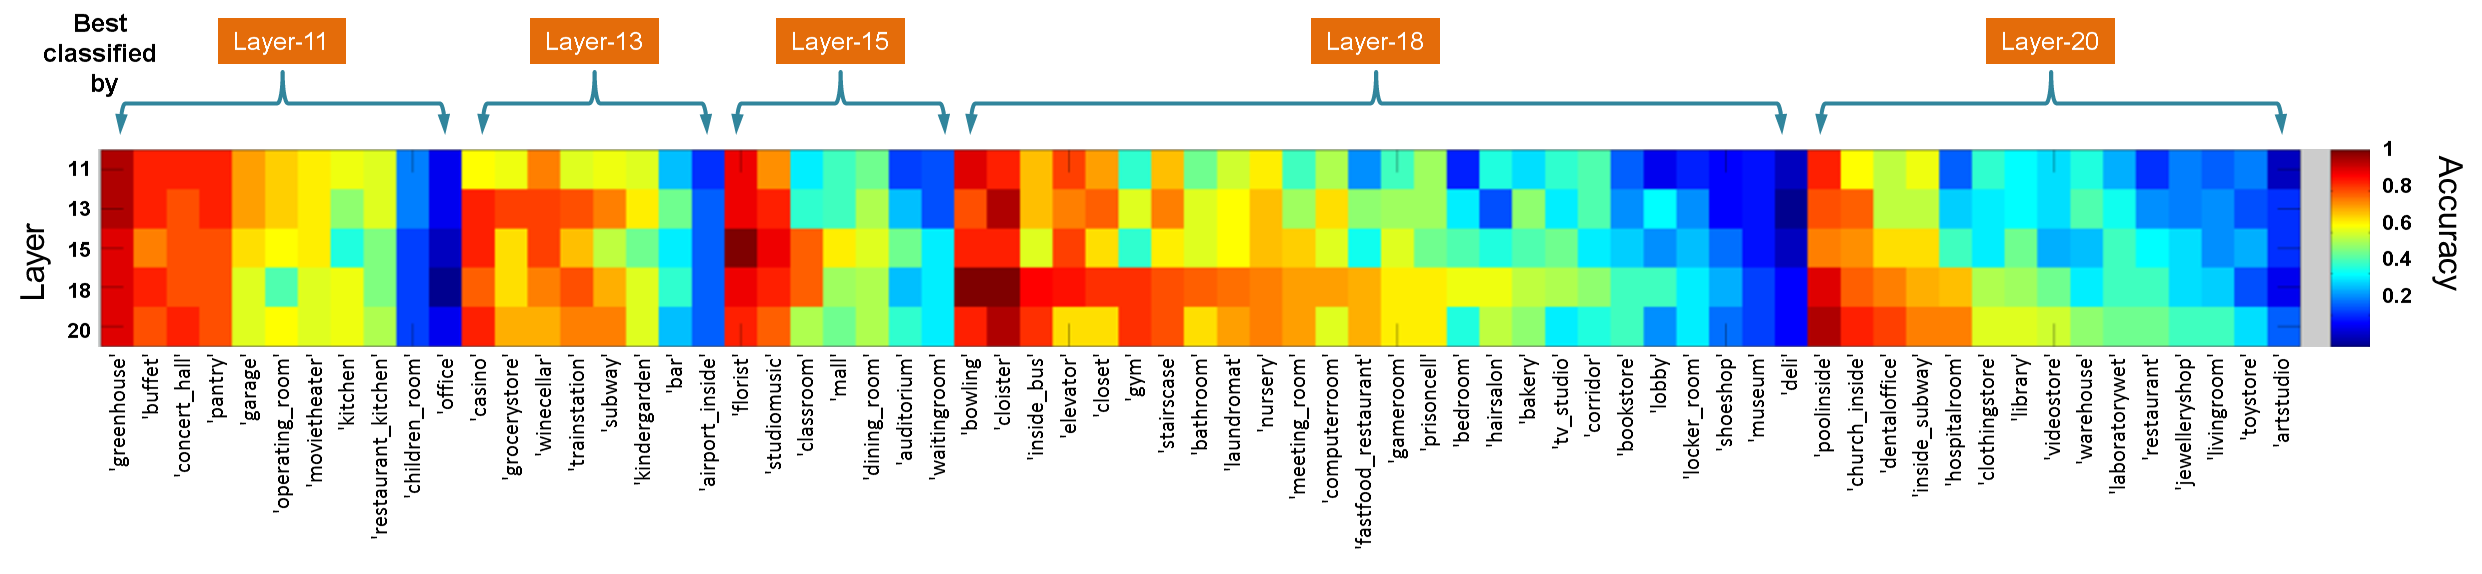
\includegraphics[width=1\textwidth]{fig/fig_level_perf}
\caption{The ``per-class'' performance using features extracted from particular layers. We group classes with identical best-performing layers. The last layer ({\bf 20}) is optimal for only 15 classes, while the second-to-last layer ({\bf 18}) proves most discriminative for 26 classes. The third-most effective layer ({\bf 11}) captures significantly lower-level level features. These results validate our underlying hypothesis; different classes require different amounts of invariance. This suggests that a feature extractor shared across such classes will be more effective when multi-scale.}
%We further analyze this phenomena in Fig.~\ref{fig:best_perf_layer_hist}.}
\label{fig:level_perf}
\end{figure*}

%\begin{figure}[t!]
%\centering
%	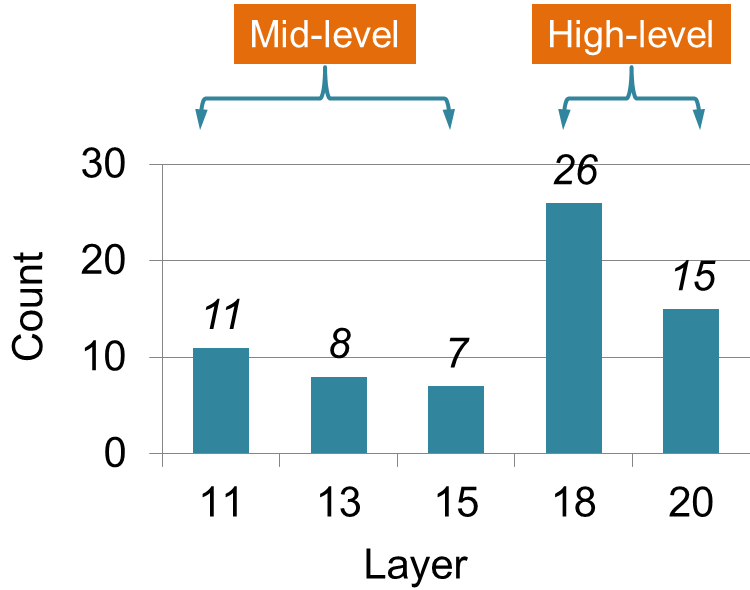
\includegraphics[width=.6\columnwidth]{fig/best_perf_layer_hist.png}
%\caption{We count the number of classes with a particular best-performing layer. The last layer ({\bf 20}) is optimal for only 15 classes, while the second-to-last layer ({\bf 18}) proves most discriminative for 26 classes. The third-most effective layer ({\bf 11}) captures significantly lower-level level features. These results validate our underlying hypothesis; different classes require different amounts of invariance. This suggests that a feature extractor shared across such classes will be more effective when multi-scale.}
% A high-level feature (Layer-18) achieves the highest accuracy in the 26 categories. In the meantime, mid-level features (Layer-11,13, and 15) are also important in this classification task. They perform the best for another 26 categories. }
%\label{fig:best_perf_layer_hist}
%\end{figure}

{\bf Scale-varying classification:} The above experiment required training $K \times N$ 1-vs-all classifiers, where $K$ is the number of classes and $N$ is the number of layers. We can treat each of the $KN$ classifiers as binary predictors, and score each with the number of correct detections of its target class. We plot these scores as a matrix in Fig.~\ref{fig:level_perf}. We tend to see groups of classes that operate best with features computed from particular high-level or mid-level layers. %Indeed, we plot the optimal scale for each binary predictor in Fig.~\ref{fig:best_perf_layer_hist}. 
Most categories tend to do well with high-level features, but a significant fraction (over a third) do better with mid-level features.

{\bf Spatial pooling:} In the next section, we will explore multi-scale features. One practical hurdle to including all features from all layers is the massive increase in dimensionality. Here, we explore strategies for reducing dimensionality through pooled features. We consider various pooling strategies (average versus max), pooling neighborhoods, and normalization post-processing (with and without L2 normalization). We saw good results with average pooling over all spatial locations, followed by L2 normalization \new{(though we will re-examine these issues further in the next section)}. Specifically, assume a particular layer is of size $H \times W \times F$, where $H$ is the height, $W$ is the width, and $F$ is the number of filter channels. We compute a $1 \times 1 \times F$ feature by averaging across spatial dimensions. We then normalize this feature to have unit norm. %Note that the ``marginal activations'' of fully-connected layers (which are already of dimension $1 \times 1 \times F$) are simply the original activations.  
%We compare this encoding versus the unpooled full-dimensional feature (also normalized) in Fig.~\ref{fig:full_marg}. Pooled features always do better, implying dimensionality reduction actually helps performance. We verified that this phenomena was due to over-fitting; the full features always performed better on training data, but performed worse on test data. This suggests that with additional training data, less-aggressive pooling (that preserves some spatial information) may perform better. %\deva{If we have time, we should explore other amounts of pooling; say pooling into quadrants such that the features is $2 \times 2 \times F$. One reviewer suggested this. This should be relatively easy to try out for single-scale. If it helps, we could try out for multi-scale and DAG.} \songfan{Please refer to email attachment for the resulting slides}

%{\bf Marginal vs full:} A reasonable question is whether some performance is sacrificed for this reduced dimensionality. To evaluate this hypothesis, we train an SVM on activations from a single layer, using both the full and marginal activations. For simplicity, we focus on the 5 best-performing layers from Fig.~\ref{fig:best_perf_layer_hist}. Surprisingly, the results in Fig.~\ref{fig:full_marg} shows that marginal features always outperform the full-dimensional feature, implying that dimensionality reduction actually helps performance. 

%\begin{figure}[t!]
%\centering
%\begin{minipage}[c]{.49\linewidth}
 % {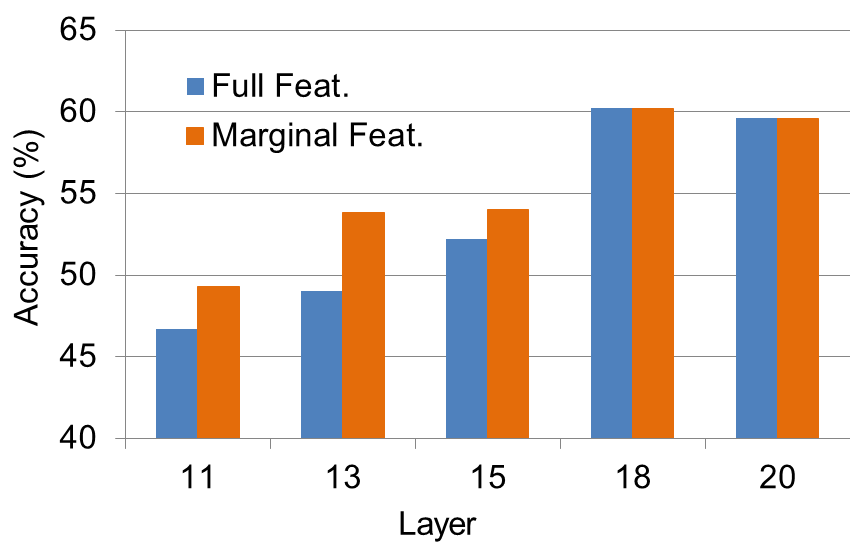
\includegraphics[width=\linewidth]{fig/full_marg.png}}
%\end{minipage}\hfill
%\begin{minipage}[c]{.51\linewidth}
%\caption{Marginal features (computed by spatially-pooling across activations from a layer) do as well or better than their full-dimensional counterpart. }
%\label{fig:full_marg}
%\end{minipage}
%\vspace{-15pt}
%\end{figure}

\subsection{Multi-scale models} 

{\bf Multi-scale classification:} We now explore multi-scale predictors that process pooled features extracted from multiple layers. As before, we analyze ``off-the-shelf'' pre-trained models. We evaluate performance as we iteratively add more layers \textcolor[rgb]{1,0,0}{by feature concatenation}. Fig.~\ref{fig:layer_MIT67} suggests that the last ReLU layer is a good starting point due to its strong single-scale performance. Fig~\ref{fig:add_back_caffe} plots performance as we add previous layers to the classifier feature set. Performance increases as we add intermediate layers, while lower layers prove less helpful (and may even hurt performance, likely do to over-fitting). Our observations suggest that high and mid-level features (\ie, \textit{parts} and \textit{objects}) are more useful than low-features based on \textit{edges} or \textit{textures} in scene classification. 


% the performance increase in the beginning by adding mid-level features to enrich the model discriminativeness. However, including some low level responses to the feature actually hurts the performance, \ie, layer 7 and 3 in Fig.~\ref{fig:add_back_caffe}. 

%Since different CNN layers correspond to image feature at various scales, seen in Fig.~\ref{fig:moti}, we wonder whether combining activations at multiple scales help to extract a better feature. To address this question, we carried out another experiments on the MIT67 data~\cite{MIT67}. We start from the average-pooled response of the last ReLU layer and greedily concatenate the ones from previous ReLU layers. The reason we start from the last ReLU layer is that, in the literature when CNN is used for feature extraction, the response of the first fully connected layer is usually selected~\cite{cnn_baseline,Gong14}. Besides, our previous analysis in Fig.~\ref{fig:layer_MIT67} also demonstrates better discriminative power of high-level CNN layer.

%The rest of the experimental setups are the same as in Sec.~\ref{sec:indi_scale}, \ie, a set of 67-way one-vs-all linear SVM classifiers are trained every time we add one more layer. Since we keep on concatenating features at lower level, the feature dimension is monotonically increasing. As the results shown in Fig.~\ref{fig:add_back}, the performance increase in the beginning by adding mid-level features to enrich the model discriminativeness. However, including some low level responses to the feature actually hurts the performance, \ie, layer 7 and 3 in Fig.~\ref{fig:add_back_caffe}. We believe it demonstrates the benefit of incorporating more discriminative mid-level and high-level features of CNN (\ie, \textit{parts} and \textit{objects}), but not necessarily the low-level features, such as \textit{edge} or \textit{textures}. 

\begin{figure}[t!]
\centering
	\subfigure[Multi-scale]{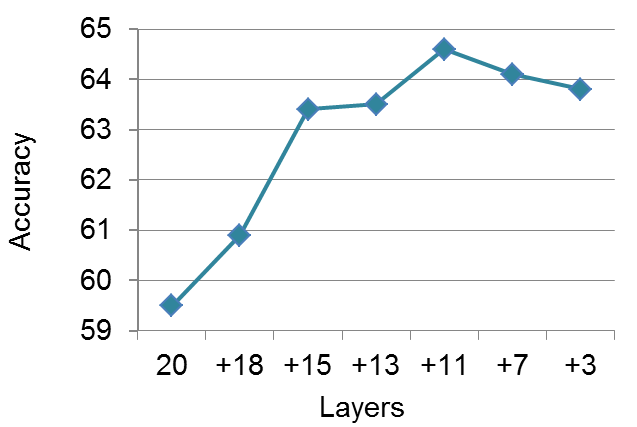
\includegraphics[width=.49\columnwidth]{fig/fig_add_back_caffe}\label{fig:add_back_caffe}}
	\subfigure[Forward Selection]{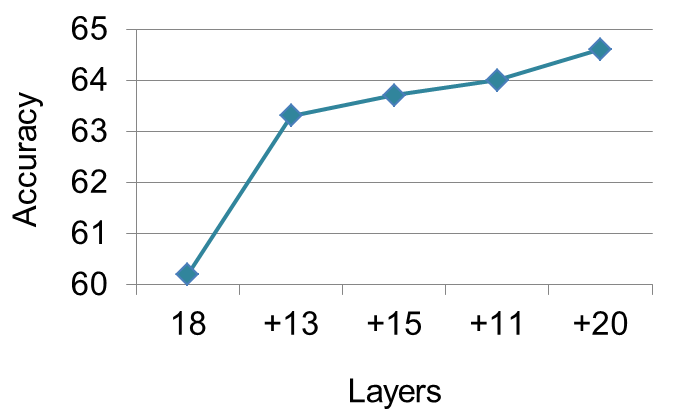
\includegraphics[width=.49\columnwidth]{fig/fig_forward_select_caffe}\label{fig:forward_select_caffe}}
\caption{ (a) The performance of a multi-scale classifier as we add more layer-specific features. We start with the last ReLU layer, and iteratively add the previous ReLU layer to the feature set of the classifier.
The ``+'' sign means the recent-most added layer. Adding additional layers help, but performance saturates and even slightly decreases when adding lower-layer features. This suggests it may be helpful to search for the ``optimal'' combination of layers. (b) The performance trend when using forward selection to incorporate the ReLU layers. Note that layers are {\em not} selected in high-to-low order. Specifically, it begin with the second-to-last ReLU layer, and skip one or more previous layers when adding the next layer. This suggests that layers encode some redundant or correlated information. Overall, we see a significant 6\% improvement.}
\label{fig:add_back}
\end{figure}

{\bf Multi-scale selection:} The previous results show that adding all layers may actually hurt performance. We verified that this was an over-fitting phenomena; additional layers always improved training performance, but could decrease test performance due to over-fitting. This appears especially true for multi-scale analysis, where nearby layers may encoded redundant or correlated information (that is susceptible to over-fitting). Ideally, we would like to search for the ``optimal'' combination of ReLU layers that maximize performance on validation data. Since there exists an exponential number of combinations ($2^N$ for $N$ ReLU layers), we find an approximate solution with a greedy forward-selection strategy. We greedily select the next-best layer (among all remaining layers) to add, until we observe no further performance improvement. As seen in Fig.~\ref{fig:forward_select_caffe}, the optimal results of this greedy approach rejects the low-level features. This is congruent with the previous results in Fig.~\ref{fig:add_back_caffe}. 

\new{{\bf Multi-scale pooling:} We use our greedy scale-selection strategy to re-examine pooling strategies. Specifically, we divide the spatial features from a particular layer into $M \times M$ non-overlapping windows, where $M$ varies from 1 to 3. We average-pool features within each window and concatenate the $M^2$ pooled features together into a final L2-normalized descriptor. When greedily searching over layers to add, we also greedily search over the 3 possible pooling windows for each layer. Interestingly, when evaluating pooling windows for {\em single-scale} classification, smaller pooling windows sometimes improved performance for certain layers. But in the multi-scale setting, there is essentially no improvement over global pooling (Fig.~\ref{fig:pool_size}), perhaps because finer spatial cues may already be captured in multi-scale features extracted from neighboring layers. We posit that with more training data, locally-pooled features may perform better. %We hypothesize that with more training data, spatial pooling may perform better.
In our subsequent analysis we consider only globally-pooled features, as they are simpler to implement and generate smaller descriptors.}
%To explore more feature concatenation strategy besides marginal features, we consider non-overlapping pooling with various window sizes in the forward selection diagnostic experiment. Concretely, we first divide the response map to $M\times M$ patches spatially. ``Sum-pooling'' and ``Max-pooling'' strategies are then applied to each patch and the resulting features are concatenated and L2 normalized. Note that the feature dimension increases at $N^2$ speed after concatenation, and thus, a large $N$ with our multi-scale feature extraction is not feasible. Here, we consider N from 1 to 4 in our experiment. As seen in Fig.~\ref{fig:pool_size}, sum-pooling is generally better than max-pooling in this task, suggesting that more aggressive max-pooling might hurt the discriminativeness of the model. Moreover, the best performance is achieved by the marginal activation with sum-pooling ($1\times 1$ in Fig.~\ref{fig:sumpool_size}), suggesting that the mean receptive field is more representative and less prone to over-fitting due to smaller feature dimension. }

\begin{figure}[t!]
\centering
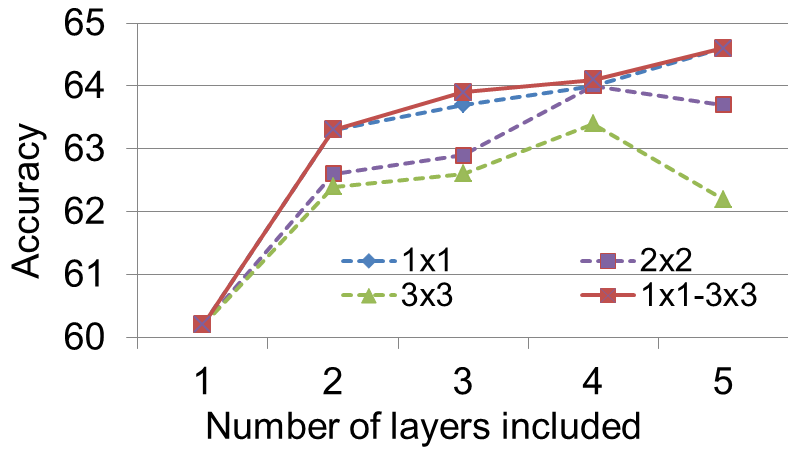
\includegraphics[width=.8\columnwidth]{fig/sumpool_size}
\caption{\new{We evaluate spatial pooling strategies to see if retaining spatial information (by pooling over smaller windows) helps multi-scale performance. The answer is essentially `no': global pooling (using a $1\times 1$ window covering the entire layer) does as well as or better than local windows, either of a fixed size or adaptive-size dynamically selected during the greedy search ({\bf all}). We posit two reasons: (1) finer spatial cues may already be captured by multiscale features extracted from neighboring layers and (2) additional training data might be needed to realize the benefit of local pooling windows since they generate larger descriptors. For reference, we also experimented with max-pooling strategies, but saw consistently worse results.}}
\label{fig:pool_size}
\end{figure}


Our analysis strongly suggest the importance (and ease) of incorporating multi-scale features for classification tasks. For our subsequent experiments, we use scales selected by the forward selection algorithm on MIT67 data (shown in Fig.~\ref{fig:forward_select_caffe}). Note that we use them for all our experimental benchmarks, demonstrating a degree of cross-dataset generalization in our approach. 

\section{Approach\label{sec:approach}} 

\begin{figure*}[t!]
\centering
	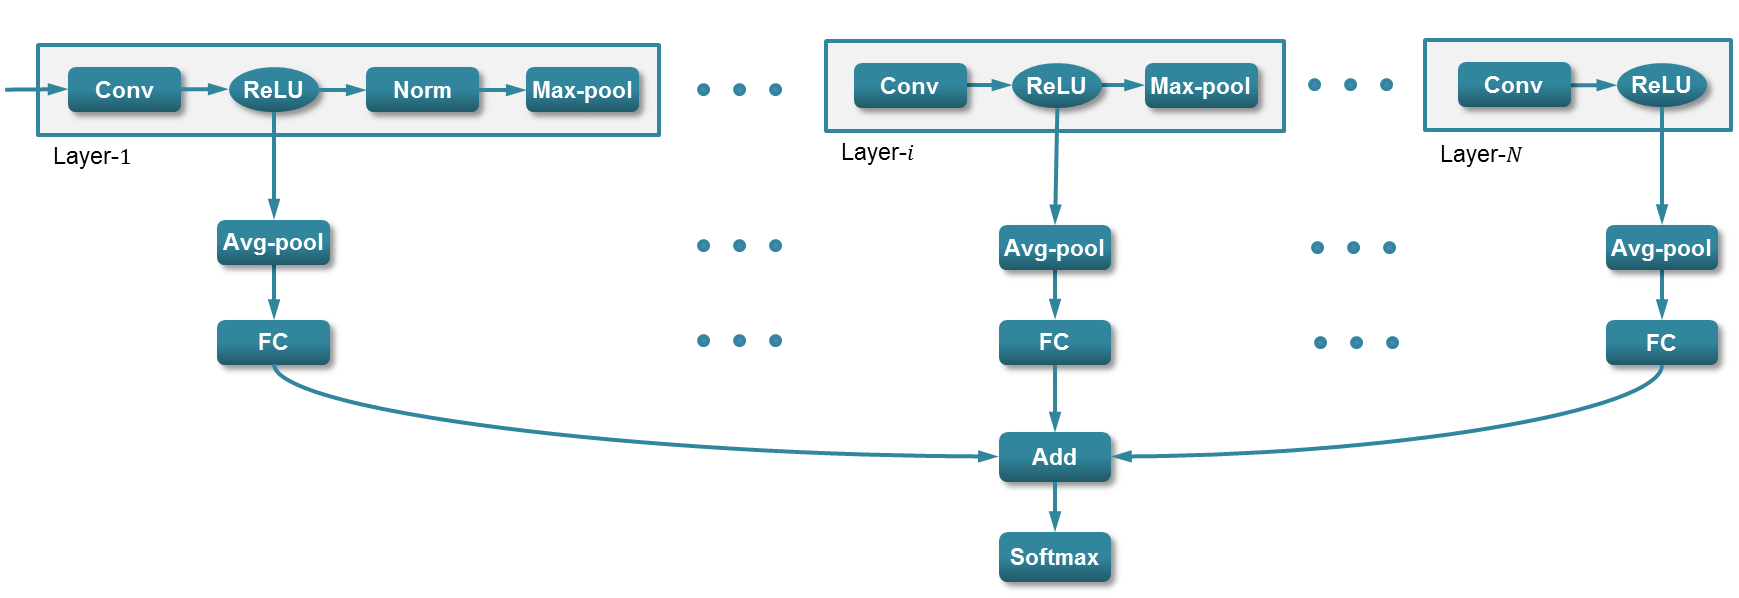
\includegraphics[width=.9\textwidth]{fig/fig_model}
\caption{Our multi-scale DAG-CNN architecture is constructed by adding multi-scale output connections to an underlying {\em chain backbone} from the original CNN. Specifically, for each scale, we spatially (average) pool activations, normalize them to have unit-norm, compute an inner product with a fully-connected (FC) layer with $K$ outputs, and add the scores across all layers to predictions for $K$ output classes (that are finally soft-maxed together).}
\label{fig:model}
\end{figure*}

In this section, we show that the multi-scale model examined in Fig.~\ref{fig:forward_select_caffe} can be written as a DAG-structured, feed-forward CNN. Importantly, this allows for end-to-end gradient-based learning. To do so, we use standard calculus constructions -- specifically the chain rule and partial derivatives -- to generalize back-propagation to layers that have multiple ``parents'' or inputs. Though such DAG structures have been previously introduced by prior work, we have not seen derivations for the corresponding gradient computations. We include them here for completeness, pointing out several opportunities for speedups given our particular structure.

{\bf Model:} The run-time behavior of our multi-scale predictor from the previous section is equivalent to feed-forward processing of the DAG-structured architecture in Fig.~\ref{fig:forward_select_caffe}. Note that we have swapped out a margin-based hinge-loss (corresponding to a SVM) with a softmax function, as the latter is more amenable to training with current toolboxes. Specifically, typical CNNs are grouped into collections of four layers, \ie, Conv., ReLU, contrast normalization (Norm), pooling layers (with the Norm and pooling layers being optional). The final layer is usually a $K$-way softmax function that predicts one of $K$ outputs. We visualize these layers as a chain-structured ``backbone'' in Fig.~\ref{fig:model}. Our DAG-CNN simply links each ReLU layer to an average-pooling layer, followed by a L2 normalization layer, which feeds to a fully-connected (FC) layer that produces $K$ outputs (represented formally as a $1 \times 1 \times K$ matrix). These outputs are element-wise added together across all layers, and the resulting $K$ numbers are fed into the final softmax function. The weights of the FC layers are equivalent to the weights of the final multi-scale $K$-way predictor (which is a softmax predictor for a softmax loss output, and a SVM for a hinge-loss output). Note that all the required operations are standard modules except for the \textit{Add}.


{\bf Training:} Let $\textbf{w}_1,...\textbf{w}_K$ be the CNN model parameters at $1,..,K$-th layer, training data be ($\textbf{x}^{(i)},\textbf{y}^{(i)}$), where $\textbf{x}^{(i)}$ is the $i$-th input image and $\textbf{y}^{(i)}$ is the indicator vector of the class of $\textbf{x}^{(i)}$. Then we intend to solve the following optimization problem
\vspace{-5pt}
\begin{align}
\argmin_{\textbf{w}_1,...\textbf{w}_K} \frac{1}{n}\sum_{i=1}^{n} \mathcal{L}(f(\textbf{x}^{(i)};\textbf{w}_1,...,\textbf{w}_K),\textbf{y}^{(i)})
\end{align}

As is now commonplace, we make use of stochastic gradient descent to minimize the objective function. For a traditional \textit{chain} model, the partial derivative of the output with respect to any one weight can be recursively computed by the chain rule, as described in the back-prop algorithm.%~\cite{rumelhart1988learning}. 

{\bf Multi-output layers (ReLU):} Our DAG-model is structurally different at the ReLU layers (since they have multiple outputs) and the \textit{Add} layer (since it has multiple inputs). We can still compute partial derivatives by recursively applying the chain rule, but care needs to be taken at these points. Let us consider the $i$-th ReLU layer in Fig.~\ref{fig:backprop_eq}. Let $\alpha_i$ be its input, $\beta_i^{(j)}$ be the output for its $j$-th output branch (its $j^{th}$ child in the DAG), and let $z$ is the final output of the softmax layer. The gradient of $z$ with respect to the input of the $i$-th ReLU layer can be computed as
\vspace{-5pt}
\begin{align}
\frac{\partial z}{\partial \alpha_i}=\sum_{j=1}^{C}\frac{\partial z}{\partial \beta_i^{(j)}}\frac{\partial \beta_i^{(j)}}{\partial \alpha_i} \quad \text {(in general)} \label{eq:backprop1}
\end{align}

\noindent where $C=2$ for the example in Fig.~\ref{fig:backprop_eq}. One can recover standard back-propagation equations from the above by setting $C=1$: a single back-prop signal $\frac{\partial z}{\partial \beta_i^{(1)}}$  arrives at ReLU unit $i$, is multiplied by the local gradient $\frac{\partial \beta_i^{(1)}}{\partial \alpha_i^{(1)}}$, and is passed on down to the next layer below. In our DAG, {\em multiple} back-prop signals arrive $\frac{\partial z}{\partial \beta_i^{(j)}}$ from each branch $j$, each is multiplied by an branch-specific gradient $\frac{\partial \beta_i^{(j)}}{\partial \alpha_i}$, and their total sum is passed on down to the next layer.

% Each partial derivative component, $\frac{\partial z}{\partial \beta_i^{(j)}}\frac{\partial \beta_i^{(j)}}{\partial \alpha_i}$, can be computed in the typical back-prop fashion. In chain-structured back-propogration, a single back-prop signal \frac{\partial z}{\partial \beta_i} will arrive at ReLU unit $i$. This is multiped by the layer-specific gradient $
%This means that during gradient updating, multiple $(C)$ backprop signals will arrive at the $i^{th}$ ReLU layer. These signals are added together, and then 

\begin{figure}[t!]
\centering
	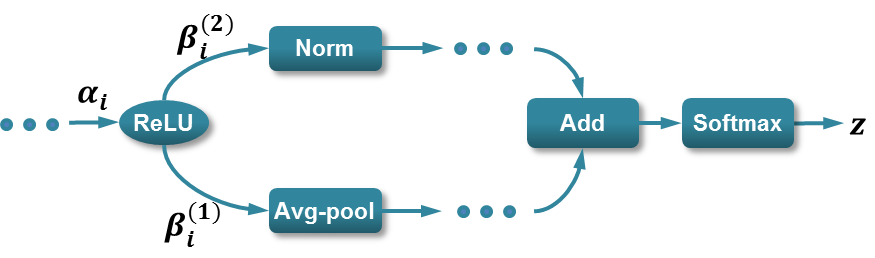
\includegraphics[width=.85\columnwidth]{fig/fig_backprop_eq}
\caption{Visualization of the parameter setup at $i$-th ReLU.}
\label{fig:backprop_eq}
\end{figure}


{\bf Multi-input layers (Add):} Let $\beta_k=g(\alpha^{(1)}_k,\cdots,\alpha^{(N)}_k)$ represents the output of a layer with multiple inputs. We can compute the gradient along the layer by applying the chain rule as follows:
\vspace{-5pt}
\begin{align}
\frac{\partial z}{\partial \alpha_i}&=\frac{\partial z}{\partial \beta_k}\frac{\partial \beta_k}{\partial \alpha_i} \nonumber \\
&=\frac{\partial z}{\partial \beta_k}\sum_{j=1}^{C}\frac{\partial \beta_k}{\partial \alpha_k^{(j)}}\frac{\partial \alpha_k^{(j)}}{\partial \alpha_i} \quad \text{(in general)} \label{eq:backprop2}
\end{align} 
One can similarly arrive at the standard back-propagation by setting $C=1$.


{\bf Special case (ReLU):} Our particular DAG architecture can further simplify the above equations. Firstly, it may be common for multiple-output layers to duplicate the same output for each child branch. This is true of our ReLU units; they pass the same values to the next layer in the chain and the current-layer pooling operation. This means the output-specific gradients are identical for those outputs $\forall j, \frac{\partial \beta_i^{(j)}}{\partial \alpha_i} =  \frac{\partial \beta_i^{(1)}}{\partial \alpha_i}$, which simplifies \eqref{eq:backprop1} to
\vspace{-5pt}
\begin{align}
\frac{\partial z}{\partial \alpha_i} = \frac{\partial \beta_i^{(1)}}{\partial \alpha_i} \sum_{j=1}^{C}\frac{\partial z}{\partial \beta_i^{(j)}} \quad \text{(for duplicate outputs)}
\end{align}
This allows us to add together multiple back-prop signals before scaling them by the local gradient, reducing 
the number of multiplications by $C$. We make use of this speed up to train our ReLU layers
. 

{\bf Special case (Add):} Similarly, our multi-input {\tt Add} layer reuses the same partial gradient for each input
$\forall j, \frac{\partial \beta_k}{\partial \alpha_k^{(j)}} = \frac{\partial \beta_k}{\partial \alpha_k^{(1)}}$ which simplifies even further in our case to $1$. The resulting back-prop equations that simplify \eqref{eq:backprop2} are given by
\vspace{-5pt}
\begin{align}
\frac{\partial z}{\partial \alpha_i} = \frac{\partial z}{\partial \beta_k} \frac{\partial \beta_k}{\partial \alpha_k^{(1)}}\sum_{j=1}^{C} \frac{\partial \alpha_k^{(j)}}{\partial \alpha_i}  \quad \text{(for duplicate gradients)}
\end{align}
\noindent implying that one can similarly save $C$ multiplications. The above equations have an intuitive implementation; the standard chain-structured back-propagation signal is simply replicated along each of the parents of the {\tt Add} layer.

{\bf Implementation:} We use the excellent MatConNet codebase to implement our modifications \cite{vedaldimatconvnet}. We implemented a custom {\tt Add} layer and a custom DAG data-structure to denote layer connectivity. Training and testing is essentially as fast as the chain model.

{\bf Vanishing gradients:} We point out an interesting property of our multi-scale models that make them easier to train. Vanishing gradients~\cite{bengio1994learning} refers to the phenomena that gradient magnitudes decrease as they are propogated through layers, implying that lower-layers can be difficult to learn because they recieve too small a learning signal. In our DAG-CNNs, lower layers are {\em directly} connected to the output layer through multi-scale connections, ensuring they receive a strong gradient signal during learning. Fig.~\ref{fig:grad} experimentally verifies this claim.

\begin{figure}[htbp]
\centering
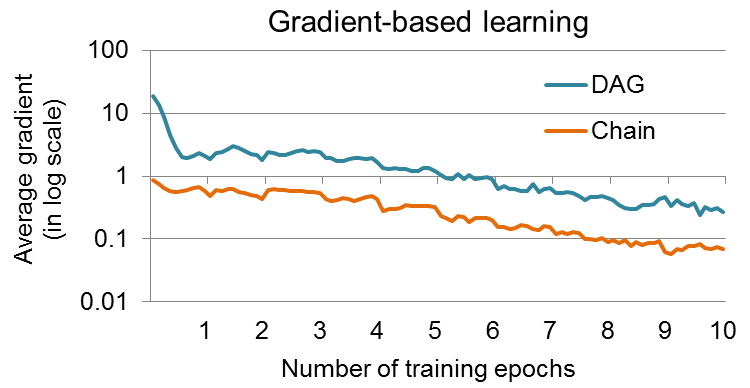
\includegraphics[width=.8\columnwidth]{fig/fig_grad}
\caption{The average gradient from Layer-1 (Conv.) during training, plotted in log-scale. Gradients from the DAG are consistently $10\times$ larger, implying that they receive a stronger supervised signal from the target label during gradient-based learning.}
\label{fig:grad}
\end{figure}


%-------------------------------------------------------------------------
%-------------------------------------------------------------------------
\section{Experimental Results\label{sec:exp}}
We explore DAG-structured variants of two popular deep models, Caffe~\cite{Caffe} and Deep19~\cite{veryDeep}. We refer to these models as Caffe-DAG and Deep19-DAG. We evaluate these models on three benchmark scene datasets: SUN397~\cite{SUN397}, MIT67~\cite{MIT67}, and Scene15~\cite{Scene15}. In absolute terms, we achieve the best performance ever reported on all three benchmarks, sometimes by a significant margin.% We also show more classification results in Fig.~\ref{fig:more_eg}. 

%\subsection{Experiment Setup}
%We stress that cross-validation on the MIT67 dataset is used to select the set of multi-scale layers in our DAG, as shown in Fig.~\ref{fig:forward_select_caffe}. The same set is then used for all other benchmark datasets. Our results may further improve through data-dependant scale selection. We explore DAG-structured variants of two popular models, Caffe~\cite{Caffe} and Deep19 models~\cite{veryDeep}. 

\begin{table*}[t!]
\centering
\resizebox{.9\textwidth}{!}{
\begin{tabular}{ccc}
SUN397 & MIT67 & Scene15\\
\begin{tabular}[t]{|l|c|}
\hline
Approach & Accuracy(\%) \\
\hline
Deep19-DAG & \textbf{56.2} \\
Deep19~\cite{veryDeep} & 51.9 \\
Caffe-DAG & 46.6	\\
Caffe~\cite{Caffe} & 43.5 \\ \hline
Places~\cite{zhoulearning} (\textcolor[rgb]{1,0,0}{Caffe})	& 54.3	\\
MOP-CNN~\cite{Gong14} (\textcolor[rgb]{1,0,0}{Caffe}) & 52.0 \\
FV~\cite{FV} & 47.2 \\
DeCaf~\cite{DeCaf} & 40.9	\\
Baseline-overfeat~\cite{SUN_ijcv}	&40.3 \\
Baseline~\cite{SUN397} & 38.0 \\
\hline
\end{tabular}
&
\begin{tabular}[t]{|l|c|}
\hline
Approach & Accuracy(\%) \\
\hline
Deep19-DAG & \textbf{77.5} \\
Deep19~\cite{veryDeep} & 70.8 \\
Caffe-DAG & 64.6	\\
Caffe~\cite{Caffe} & 59.5 \\ \hline
MOP-CNN~\cite{Gong14} (\textcolor[rgb]{1,0,0}{Caffe}) & 68.9 \\
Places~\cite{zhoulearning} (\textcolor[rgb]{1,0,0}{Caffe})	& 68.2	\\
Mid-level~\cite{mid_level} & 64.0	\\
FV+BoP~\cite{FV_BoP} & 63.2 \\
Disc. Patch~\cite{disc_patch} & 49.4 \\
SPM~\cite{spatial_pyramid} & 34.4	\\
\hline
\end{tabular}
&
\begin{tabular}[t]{|l|c|}
\hline
Approach & Accuracy(\%) \\
\hline
Deep19-DAG & \textbf{92.9} \\
Deep19~\cite{veryDeep} & 90.8 \\
Caffe-DAG & 89.7	\\
Caffe~\cite{Caffe} & 86.8 \\ \hline
Place~\cite{zhoulearning} (\textcolor[rgb]{1,0,0}{Caffe}) & 91.6 \\
CENTRIST~\cite{Wu_pami11} & 84.8	\\
Hybrid~\cite{Bosch_pami08}	& 83.7	\\
Spatial pyramid~\cite{spatial_pyramid} & 81.4 \\
Object bank~\cite{Li_nips10_objectbank}	& 80.9	\\
Reconfigurable model~\cite{Parizi_cvpr12_reconf} & 78.6	\\
Spatial Envelop~\cite{Oliva_ijcv01_envelop} & 74.1 \\
Baseline~\cite{Scene15} & 65.2 \\
\hline
\end{tabular}
\end{tabular}
}
\caption{Classification results on SUN397, MIT67, and Scene15 datasets. \new{We explicitly denote those methods that make use of the same Caffe model, either applied with a different (multi-scale) post-processing stage~\cite{Gong14} or learned with a massively-large custom dataset~\cite{zhoulearning}.} Please see text for an additional discussion.}
\label{table:all}
\end{table*}


{\bf Feature dimensionality:} Most existing methods that use CNNs as feature extractors work with the last layer (or the last fully connected layer), yielding a feature vector of size 4096. 
Forward feature selection on Caffe-DAG selects layers $(11, 13, 15, 18, 20)$, making the final multi-scale feature 9216-dimensional. Deep19-DAG selects layers$( 26, 28, 31, 33, 30)$, for a final size of 6144. We perform feature selection by cross-validating on MIT67, and use the same multi-scale structure for all other datasets. Dataset-dependant feature selection may further improve performance. Our final multi-scale DAG features are {\em only 2X larger} than their single-scale counter part, making them practically easy to use and store.


{\bf Training:}  We follow the standard image pre-processing steps of fixing the input image size to $224\times 224$ by scaling and cropping, and subtracting out the mean RGB value (computed on ImageNet). We initialize filters and biases to their pre-trained values (tuned on ImageNet) and initialize multi-scale fully-connected (FC) weights to small normally-distributed numbers. We perform 10 epochs of learning.

{\bf Baselines:} We compare our DAG models to published results, including two additional baselines. We evaluate the best single-scale ``off-the-shelf'' model, using both Caffe and Deep19. We pass L2-normalized single-scale features to Liblinear~\cite{liblinear} to train $K$-way one-vs-all classifiers with default settings. Finally, Sec.~\ref{sec:diag} concludes with a detailed diagnostic analysis comparing off-the-shelf and fine-tuned versions of chain and DAG structures.

%-------------------------------------------------------------------------


\begin{figure*}[t!]
\centering
	\includegraphics[width=.9\textwidth]{fig/fig_more_eg}
\caption{Deep19-DAG results on MIT67. The category label is shown on the left and the label for false-positives (in {\bf red}) are also provided. We use the multi-scale analysis of Fig.~\ref{fig:level_perf} to compare categories that perform better with mid-level features ({\bf top 2 rows}) versus high-level features ({\bf bottom 2 rows}). Mid-level features appear to emphasize \textit{objects} such as operating equipment for {\tt operating room} scenes and circular grid for {\tt  wine celler}, while high-level features appear to focus on global \textit{spatial statistics} for {\tt inside bus} and {\tt elevator} scenes. }%\songfan{showing a different set of results. The selected classes all have large performance difference for mid- vs high-level features, based on Fig. 4.}}
\label{fig:more_eg}
\end{figure*}

{\bf SUN397:} We tabulate results for all our benchmark datasets in Table~\ref{table:all}, and discuss each in turn. SUN397~\cite{SUN397} is a large scene recognition dataset with 100K images spanning 397 categories, provided with standard train-test splits. Our DAG models outperform their single-scale counterparts. In particular, Deep19-DAG achieves the highest $56.2\%$ accuracy. Our results are particularly impressive given that the next-best method of~\cite{zhoulearning} (with a score of $54.3$) makes use of a ImageNet-trained CNN and a custom-trained CNN using a new 7-million image dataset with 400 scene categories.



%-------------------------------------------------------------------------
%\subsection{MIT67}

{\bf MIT67:} MIT67 consists of 15K images spanning 67 indoor scene classes~\cite{MIT67}, provided with standard train/test splits. Indoor scenes are interesting for our analysis because some scenes are well characterized by high-level spatial geometry (\eg~{\tt church} and {\tt cloister}), while others are better described by mid-level objects (\eg~{\tt wine celler} and {\tt operating room}) in various spatial configurations. We show qualitative results in Fig.~\ref{fig:more_eg}. Deep19-DAG produces a classification accuracy of $77.5\%$, reducing the best-previously reported error~\cite{Gong14} by {\bf 23.9\%}. Interestingly~\cite{Gong14} also uses multi-scale CNN features, but do so by first extracting various-sized patches from an image, rescaling each to canonical size. Single-scale CNN features extracted from these patches are then vector-quantized into a large-vocabulary codebook, followed by a projection step to reduce dimensionality. Our multi-scale representation, while similar in spirit, is an end-to-end trainable model that is computed ``for free'' from a single (DAG) CNN.

%Our DAG-CNN model is designed to encode features across multiple scales and capture high- and mid-level statistics of scene categories. Similar observations can be drawn from Table.~\ref{table:all}. The DAG-CNN models consistently out-perform the traditional chain model. The highest accuracy, $77.5\%$ is achieved by the DAG-CNN with a Deep19 backbone. Our results reduce the best-previously reported error~\cite{Gong14} by {\bf 23.9\%}. Interestingly~\cite{Gong14} also uses multi-scale CNN features, but do so by first extracting various-sized patches from an image, rescaling each to canonical size. Single-scale CNN features extracted from these patches are then vector-quantized into a large-vocabulary codebook, followed by a projection step to reduce dimensionality. Our multi-scale representation, while similar in spirit, is an end-to-end trainable model that is computed ``for free'' from a single (DAG) CNN.
% The activation of first fully connected layer is concatenated. Their method is less efficient to the the multiple runs of feed-forward computation and high dimensional features.


%-------------------------------------------------------------------------
%\subsection{Scene15}

{\bf Scene15:} The Scene15~\cite{Scene15} includes both indoor scene (\eg, store and kitchen) and outdoor scene (\eg, mountain and street). It is a relatively small dataset by contemporary standards (2985 test images), but we include here for completeness. Performance is consistent with the results above. Our multi-scale DAG model, specifically Deep19-DAG, outperforms all prior work. For reference, the next-best method of~\cite{zhoulearning} uses a new custom 7-million image scene dataset for training.

%A 10-fold split is provided with 1500 training and 2985 test image, where all images come in black and white. A consistent performance also is observed in Table.~\ref{table:all}. 

%-------------------------------------------------------------------------
%-------------------------------------------------------------------------

\subsection{Diagnostics \label{sec:diag}}
In this section, we analyze ``off-the-shelf'' (OTS) and ``fine-tuned'' (FT) versions of both single-scale chain and multi-scale DAG models. We focus on the Caffe model, as it is faster and easier for diagnostic analysis. 

{\bf Chain:} Chain-OTS uses single-scale features extracted from CNNs pre-trained on ImageNet. These are the baseline Caffe results presented in the previous subsections. Chain-FT trains a model on the target dataset, using the pre-trained model as an initialization. This can be done with standard software packages~\cite{vedaldimatconvnet}. To ensure consistency of analysis, in both cases features are passed to a K-way multi-class SVM to learn the final predictor. %We saw a small improvement in performance in doing this, rather than directly using the softmax prediction.

{\bf DAG:} DAG-OTS is obtained by fixing all internal filters and biases to their pre-trained values, and only learning the multi-scale fully-connected (FC) weights. Because this final stage learning is a convex problem, this can be done by simply passing off-the-shelf multi-scale features to a convex linear classification package (e.g., SVM). We compare this model to a fine-tuned version that is trained end-to-end, making use of the modified backprop equation from Sec.~\ref{sec:approach}. %We will show that off-the-shelf DAGs perform quite well, though fine-tuning does further improve performance.

{\bf Comparison:} Fig.~\ref{fig:comp_otf} compares off-the-shelf and fine-tune variants of chain and DAG models. We see two dominant trends. First, as perhaps expected, fine-tuned (FT) models consistently outperform their off-the-shelf (OTS) countparts. Even more striking is the large improvement from chain to DAG models, indicating the power of multi-scale feature encodings.

{\bf DAG-OTS:} Perhaps most impressive is the strong performance of DAG-OTS. From a theoretical perspective, this validates our underyling hypothesis that multi-scale features allow for better transfer between recognition tasks -- in this case, ImageNet and scene classification. An interesting question is whether multi-scale features, when trained with gradient-based DAG-learning on ImageNet, will allow for even more transfer. We are currently exploring this. However even with current CNN architectures, our results suggest that {\em any system making use of off-the-shelf CNN features should explore multi-scale variants as a ``cheap" baseline.}  Compared to their single-scale counterpart, multi-scale features require no additional time to compute, are only a factor of 2 larger to store, and consistently provide a noticeable improvement.


\begin{figure}[t]
\centering
	\subfigure[SUN397]{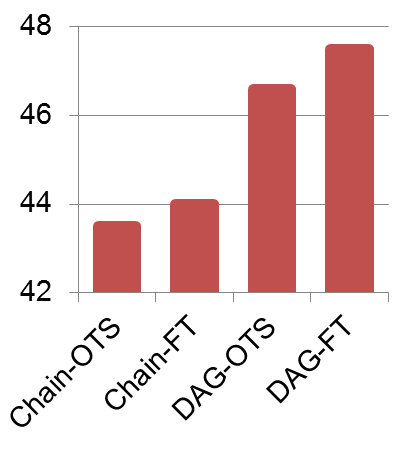
\includegraphics[width=.32\columnwidth]{fig/comp_sun}\label{fig:comp_sun}}
	\subfigure[MIT67]{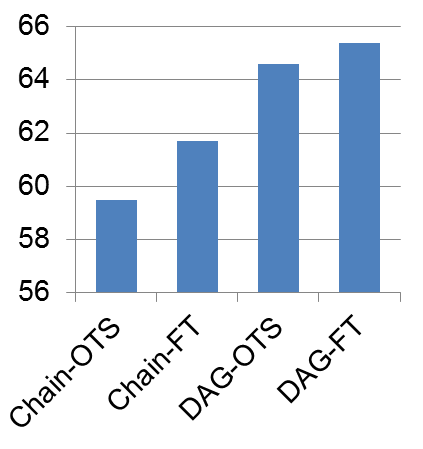
\includegraphics[width=.32\columnwidth]{fig/comp_mit}\label{fig:comp_mit}}
	\subfigure[Scene15]{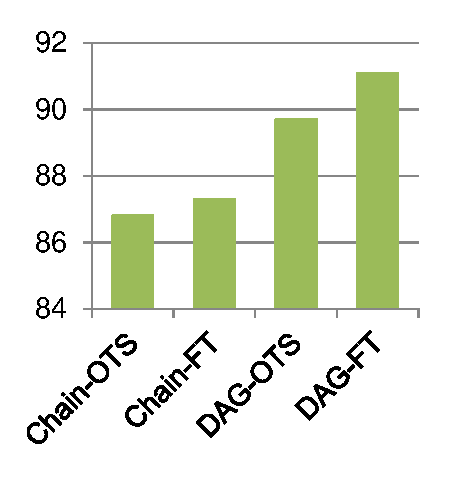
\includegraphics[width=.32\columnwidth]{fig/comp_scene}\label{fig:comp_scene}}
	
\caption{Off-the-shelf vs. Fine-tuning models on both Chain and DAG model for Caffe backbone. Please see the text for a discussion.}
\label{fig:comp_otf}
\end{figure}


%-------------------------------------------------------------------------
%-------------------------------------------------------------------------
%\section{Conclusion}

{\bf Conclusion:} We have introduced multi-scale CNNs for image classification. Such models encode scale-specific features that can be effectively shared across both coarse and fine-grained classification tasks. Importantly, such models can be viewed as DAG-structured feedforward predictors, allowing for end-to-end training. While fine-tuning helps performance, we empirically demonstrate that even ``off-the-self'' multi-scale features perform quite well. We present extensive analysis and demonstrate state-of-the-art classification performance on three standard scene benchmarks, sometimes improving upon prior art by a significant margin. %\deva{We need to get main text and figures into 8 pages, and all references into 1}.
\newpage
{\small
\bibliographystyle{ieee}
\bibliography{mobib}
}
%When placing figures in \LaTeX, it's almost always best to use
%\verb+\includegraphics+, and to specify the  figure width as a multiple of
%the line width as in the example below
%{\small\begin{verbatim}
   %\usepackage[dvips]{graphicx} ...
   %\includegraphics[width=0.8\linewidth]
                   %{myfile.eps}
%\end{verbatim}
%}


\end{document}

%%% Local Variables:
%%% mode: latex
%%% TeX-master: t
%%% End:
